\begin{DoxyAuthor}{Author}
Olha Sereda 
\end{DoxyAuthor}
\begin{DoxyDate}{Date}
2022 
\end{DoxyDate}
\begin{DoxyCopyright}{Copyright}
Olha Sereda (\href{mailto:olha.sereda@student.uj.edu.pl}{\texttt{ olha.\+sereda@student.\+uj.\+edu.\+pl}})
\end{DoxyCopyright}
Example of the snake game with using SFML Library~\newline
The main goal of the game is eating the green apples and avoid of walls and self intersection.~\newline
~\newline
Usage keys\+:~\newline
{\bfseries{Left arrow key}} -\/ turn direction counterclock-\/wise. Continius key pressing accelerates the speed of turn.~\newline
{\bfseries{Right arrow key}} -\/ turn direction clockwise. Continius key pressing accelerates the speed of turn.~\newline
{\bfseries{Up arrow key}} -\/ restarts the level after the snake die.~\newline
~\newline
 
\begin{DoxyInlineImage}
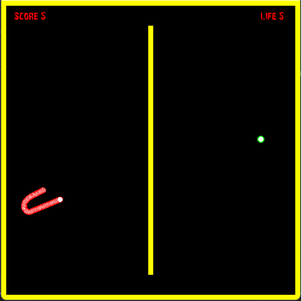
\includegraphics[height=\baselineskip,keepaspectratio=true]{snake1.png}%Snake game process
\end{DoxyInlineImage}
     
\begin{DoxyInlineImage}
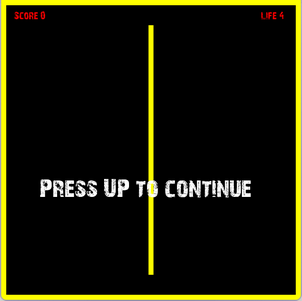
\includegraphics[height=\baselineskip,keepaspectratio=true]{snake2.png}%Snake game process
\end{DoxyInlineImage}
    ~\newline
~\newline
~\newline
File {\bfseries{levels.\+txt}} contains level\textquotesingle{}s diagaram\+:~\newline
level contains keyword {\bfseries{Level\#XX}} at begin -\/ where XX is index number~\newline
Then contains list of box coordinated -\/ {\bfseries{each line contains one set of wall coodinates}}.~\newline
and then level description ends by \textquotesingle{}\#\#\#\textquotesingle{} string.~\newline
~\newline
Example\+: 
\begin{DoxyCode}{0}
\DoxyCodeLine{Level\#1}
\DoxyCodeLine{0 590 600 10}
\DoxyCodeLine{0 0 10 600}
\DoxyCodeLine{590 0 10 600}
\DoxyCodeLine{0 0 600 10}
\DoxyCodeLine{\textcolor{preprocessor}{\#\#\#}}
\DoxyCodeLine{Level\#2}
\DoxyCodeLine{0 590 600 10}
\DoxyCodeLine{0 0 10 600}
\DoxyCodeLine{590 0 10 600}
\DoxyCodeLine{0 0 600 10}
\DoxyCodeLine{295 50 10 500}
\DoxyCodeLine{\textcolor{preprocessor}{\#\#\#}}
\DoxyCodeLine{Level\#3}
\DoxyCodeLine{0 590 600 10}
\DoxyCodeLine{0 0 10 600}
\DoxyCodeLine{590 0 10 600}
\DoxyCodeLine{0 0 600 10}
\DoxyCodeLine{295 50 10 500}
\DoxyCodeLine{50 295 500 10}
\DoxyCodeLine{\textcolor{preprocessor}{\#\#\#}}

\end{DoxyCode}
 ~\newline
The game uses \href{https://www.sfml-dev.org/}{\texttt{ SFML}} library. 